\documentclass[a4paper]{article}
%\usepackage[14pt]{extsizes}
\usepackage[T2A]{fontenc}
\usepackage[utf8]{inputenc}
\usepackage[english,russian]{babel}
\usepackage{geometry}
\usepackage{indentfirst}
\usepackage{enumerate}
\usepackage{tabularx}
\geometry{left=3.5cm}
\geometry{right=1.5cm}
\geometry{top=2cm}
\geometry{bottom=2cm}
\linespread{1.3}
\usepackage{parskip}
\makeatletter
\renewcommand{\@biblabel}[1]{#1.}
\renewcommand\contentsname{Projects List}
\makeatother
\addto\captionsrussian{\def\refname{Литература}}
\usepackage[final]{graphicx}
\graphicspath{{image/}}
%нумерация страниц
\usepackage{fancyhdr}
\pagestyle{fancy}
\fancyhf{}
\fancyfoot[R]{\thepage}
\fancyheadoffset{0mm}
\fancyfootoffset{0mm}
\setlength{\headheight}{17pt}
\renewcommand{\headrulewidth}{0pt}
\renewcommand{\footrulewidth}{0pt}
\fancypagestyle{plain}{ 
    \fancyhf{}
    \rhead{\thepage}}

%\sloppy
\usepackage{titlesec}
  \newpagestyle{kmvmain}[\small]{
    \setfoot[]%even-left
            []%even-center
            []%even-right
            {}%odd-left
            {\large{Челябинск-2018}}%odd-center
            {}%  odd-right
}
\usepackage{setspace}
\begin{document}
\begin{article}

\thispagestyle{kmvmain}
\begin{center}

\large{
МИНИСТЕРСТВО ОБРАЗОВАНИЯ И НАУКИ РОССИЙСКОЙ ФЕДЕРАЦИИ}
\Large{Федеральное государственное автономное образовательное \\ 
учреждение высшего образования}

\Large{\textbf{
"Южно-Уральский государственный университет \\ 
(национальный исследовательский университет)" \\ 
Высшая школа электроники и компьютерных наук \\ 
Кафедра системного программирования}}\\

\vspace{1.5cm}

\Large{\textbf{
Разработка игры <<Монополия>> с использованием нейросетевых технологий}}

\vspace{1.5cm}

\Large{КУРСОВАЯ РАБОТА \\ 
по дисциплине «Программная инженерия» \\ 
ЮУрГУ – 02.03.02.2018.115-083.КР}

\vspace{1cm}
\end{center}

\begin{onehalfspace}
\Large
\begin{tabular}{ll}
Нормоконтроллер, \hspace{1cm}& Научный руководитель: \\
Преподаватель кафедры СП \hspace{1cm}& Преподаватель кафедры СП \\
\underline{\hspace{3cm}}М.С. Тимченко \hspace{1cm} & \underline{\hspace{3cm}}М.С. Тимченко \\
``\underline{\hspace{0.5cm}}''\underline{\hspace{3cm}}2018 г. \hspace{1cm} & \\
\hspace{1cm}& Автор работы: \\
\hspace{1cm}& студент группы КЭ-301 \\
\hspace{1cm}& \underline{\hspace{3cm}}А.А. Бурулев \\
&\\
&\\
& Работа защищена \\
& с оценкой: \underline{\hspace{3cm}} \\
& ``\underline{\hspace{0.5cm}}''\underline{\hspace{3cm}}2018 г.\\
\end{tabular}\
\end{onehalfspace}
\end{article} 




\newpage

\begin{article}
\begin{center}

\large{
МИНИСТЕРСТВО ОБРАЗОВАНИЯ И НАУКИ РОССИЙСКОЙ ФЕДЕРАЦИИ}
\Large{Федеральное государственное автономное образовательное \\ 
учреждение высшего образования}

\Large{\textbf{
"Южно-Уральский государственный университет \\ 
(национальный исследовательский университет)" \\ 
Высшая школа электроники и компьютерных наук \\ 
Кафедра системного программирования}}\\

\vspace{0.5cm}

\begin{tabular}{ll}
\hspace{9cm} & УТВЕРЖДАЮ \\
& Зав. кафедрой СП \\
& \underline{\hspace{3cm}}Л.Б. Соколинский \\
& <<\underline{\hspace{0.5cm}}>>\underline{\hspace{3cm}}2018
\end{tabular}\

\vspace{1cm}

\Large{\textbf{
ЗАДАНИЕ \\ 
на выполнение курсовой работы} \\
по дисциплине <<Программная инженерия>> \\
студенту группы КЭ-301 \\
Бурулеву Антону Александровичу, \\
обучающемуся по направлению \\
02.03.02 «Фундаментальная информатика и информационные технологии» \\
}

\vspace{0.5cm}


\end{center}

\Large{
\begin{enumerate}
    \item[\textbf{1.}] \textbf{Тема работы}\\
    Разработка игры <<Монополия>> с использованием нейросетевых технологий
    \item[\textbf{2.}] \textbf{Срок сдачи студентом законченной работы:} 31.05.2018 г.
    \item[\textbf{3.}] \textbf{Исходные данные к работе}
    \begin{enumerate}
        \item [1.] Tariq Rashid. Make your own neural network, 2015. -240 p.
        \item [2.] Mnih, Volodymyr, Kavukcuoglu, Koray, Silver, David, Graves, Alex, Antonoglou, Ioannis, Wierstra, Daan, and Riedmiller, Martin. Playing atari with deep reinforcement learning // NIPS Deep Learning Workshop, 2013., pp. 1-9.
        \item [3.] Стюарт Р., Питер Н. Искусственный интеллект: Современный подход // Интеллектуальные агенты. 2-е издание. М.: Вильямс, 2006. С. 75-109.
    \end{enumerate}
    \item[\textbf{4.}] \textbf{Перечень подлежащих разработке вопросов}
    \begin{enumerate}
        \item [1.] Изучение методов обучения нейронных сетей
        \item [2.] Обзор используемых технологий
        \item [3.] Разработка игры <<Монополия>>
        \item [4.] Реализация нейронной сети для разработанной игры
        \item [5.] Тестирование полученной программы
    \end{enumerate}
\end{enumerate}
}
\textbf{Дата выдачи задания:} «9» февраля 2018 г.\\

\begin{onehalfspace}
\Large
\begin{tabular}{l{0.5\linewidth}l{0.5\linewidth}}
Научный руководитель \hspace*{5cm}& М.С. Тимченко \\
Преподаватель кафедры СП, \hspace{2cm}& \\
НИУ ЮУрГУ \hspace{2cm}& \\
\end{tabular}\
\end{onehalfspace}
\vspace{1cm}
\begin{onehalfspace}
\Large
\begin{tabular}{l{0.5\linewidth}l{0.5\linewidth}}
Задание принял к исполнению \hspace*{4.5cm}& А.А. Бурулев \\
\end{tabular}\
\end{onehalfspace}

\end{article} 

\newpage
\begin{Large}
\begin{spacing}{0.9}
    \tableofcontents 
    \end{spacing}
    \end{Large}

\setlength{\parskip}{0cm}
\begin{Large}
\newpage
\section*{Введение}
\addcontentsline{toc}{section}{Введение}
\textbf{Актуальность темы}

На данный момент основными способами разработки искусственного интеллекта для различных игр является конечный автомат и дерево вариантов [10]. С развитием науки и увеличением мощности вычислительной техники стало популярным машинное обучение, в частности нейронные сети. Стандартные способы обучения плохо подходят для разработки искусственного интеллекта из-за необходимости составлять обучающую выборку, что является трудоёмкой задачей для больших игр. Для таких задач отлично подходит метод обучения с подкреплением. 

Создание самообучающихся алгоритмов на основе Reinforcement Learning (Обучение с подкреплением) является актуальной задачей в современном мире, поскольку данный метод работает без заранее подготовленных ответов. Эта способность данного метода открывает возможности для решения нового вида задач. В частности, этот метод используется для обучения компьютеров прохождению игр. Создание подобных самообучающихся алгоритмов имеет важное практическое и научное значение, поскольку такие алгоритмы могут послужить основой для дальнейших исследований и совершенствований для создания алгоритмов, решающих реальные задачи. 

\textbf{Цели и задачи работы}

Целью данной работы является разработка игры «Монополия» с использованием нейросетевых технологий.

Основные задачами работы следующие:
\begin{spacing}{0.9}
\begin{enumerate}
    \item Изучение методов обучения нейронных сетей
    \item Обзор используемых технологий
    \item Разработка игры «Монополия»
    \item Реализация нейронной сети для разработанной игры
    \item Тестирование полученной программы
\end{enumerate}
\end{spacing}
\end{Large}
\newpage
\setlength{\parskip}{0cm}
\begin{Large}
\section{Анализ предметной области}
\subsection{Анализ аналогичных проектов}
В основе нейросетевых технологий лежит принцип искусственных нейронных сетей. Искусственная нейронная сеть - математическая модель, а также её программное или аппаратное воплощение, построенная по принципу организации и функционирования биологических нейронных сетей — сетей нервных клеток живого организма. Нейронные сети не программируются в привычном смысле этого слова, они обучаются. Возможность обучения — одно из главных преимуществ нейронных сетей перед традиционными алгоритмами. Технически обучение заключается в нахождении коэффициентов связей между нейронами[8]. Однако существует множество способов обучения нейронных сетей. 

Так, в одной статье рассматривается модель нейронной сети, имитирующей логику противника в игре «крестики-нолики»[1]. Структура разработанной сети состоит из одного входного нейрона, промежуточного слоя, состоящего из девяти нейронов, каждый из которых отвечает за клетку на поле, и выходного нейрона. Каждый промежуточный нейрон имеет свое весовое значение в пределах от - 1 до 1, от которого зависит выбор клетки для хода. Сеть оценивает каждую свободную клетку и выбирает наиболее перспективную. Обучающая выборка состоит из наборов заранее записанных ходов против сети. Нейронная сеть играет против каждого набора до тех пор, пока не выиграет. Процесс обучения состоит в том, что перед началом матча нейронная сеть генерирует значения весов. Исходя из этих значений и свободных клеток, сеть делает свои ходы, если она проигрывает игру значения весов, которые соответствуют произведенным ходам, уменьшаются. Если сеть выигрывает игру, значения весов увеличиваются, и игра записывается в память. Если сеть играет в ничью, то значения весов не изменяются, игра записывается в память, но дополнительно играет еще три раза с новыми значениями весов, для проверки возможности других комбинаций ходов. Процесс выбора связан с обращением сети к ее памяти значений весов. Находится игра из памяти, где противником были сделаны ходы, сделанные в текущей игре, но сеть при этом выиграла. Выбирается наиболее приближенное к единице значение весов, которое затем конвертируется в клетку. Автор отмечает что, если оппонент специально не поддаётся сети, то исходом матчей будет являться ничья, как и в случае, если нейронная сеть будет играть против такой же нейронной сети.

В другой статье рассматривается реализация поведения агента в мультиагентной компьютерной игре[4]. Игра “Collector Stars” представляет собой двумерную игру в жанре платформер для одного или нескольких игроков. Игра представлена двумерной сеткой ячеек разного типа: проходимая, непроходимый блок, звезда, черная дыра и дверь. Персонажу Собирателю нужно найти выход из уровня, попутно собирая звезды и избегая черных дыр. Агент-собиратель может перемещаться влево или вправо и прыгать на высоту, чуть выше, чем высота одной ячейки карты.  Имеет меньшие размеры по ширине и высоте, чем размер ячейки.

На вход искусственной нейронной сети подается набор атрибутов текущего состояния. Значение первого входа зависит от того, находится ли персонаж на блоке, и может иметь значение ноль или единица. Второй и третий входы представляют значения компонент нормированного вектора скорости Собирателя. Третий и четвертый входы представляют значения компонент нормированного вектора направления ближайшего противника. Пятый и шестой - координаты центра Собирателя относительно ячейки, в которую входит точка центра. Координаты нормируются с учетом размера ячейки. Далее следуют входы, представляющие ячейки вокруг собирателя, их количество определялось при тестировании. Выходом сети будут три значения, исходя из которых будут определены действия Собирателя: движение влево, вправо и прыжок, соответственно. Действие будет активизировано, если полученное значение больше 0.5.
\subsection{Обзор методов обучения нейронной сети}
Обучение на основе учебной выборки для игры в монополию невозможно, ввиду огромного количества вариантов развития. Однако существуют другие варианты обучения нейронной сети. Так в статье[4] был выбран эволюционный подход с помощью генетического алгоритма. Для обучения таким способом гены хромосом определяются как вес всех связей нейронной сети. На этапе инициализации хромосомы заполняются случайными вещественными числами из интервала [-1,1]. Агент использует значения хромосом для задания весов сети. Для определения приспособленности каждой хромосомы агенту дается некоторое время на прохождение уровня. Агент будет проходить уровень столько раз, сколько хромосом в популяции. После окончания времени, гибели или пересечения двери, приспособленность определяется как количество набранных очков. Причем если Собиратель погиб, очки все равно будут вычисляться по этой формуле, но будет использоваться количество итераций, даваемое на прохождение. После вычисления приспособленности, выполняются остальные шаги алгоритма.

Селекция или выбор родителей: метод рулетки. Каждой хромосоме сопоставляется значение, величина которого устанавливается пропорционально значению приспособленности данной хромосомы. Чем больше значение приспособленности, тем больше вероятность ее выбора.

Скрещивание и мутация: скрещивание выполняется одноточечным обменом, мутация для каждого гена происходит с вероятностью 0.01. Значение гена меняется путем прибавления случайного числа из отрезка [-0.3; 0.3] и ограничивается отрезком [-1;1].

Выбор следующего поколения: из старого поколения берется 0.6 лучших по приспособленности особей. Они объединяются с полученными потомками, но с сохранением размера популяции (т. е. часть потомков не попадет в новое поколение).

Автор приводит сравнение с другими алгоритмами, из которых видно, что нейронная сеть набирает наибольшее количество очков, однако обучается и проходит уровень чуть дольше чем алгоритм R-Learning.

Помимо лучшей скорости обучения, алгоритм Reinforcement Learning превосходно подходит для случаев, где рассматриваемая система является марковским случайным процессом, то есть процессом «будущее» которого не зависит от «прошлого» при известном «настоящем». Основная идея reinforcement learning описана в статье[6]. Авторы рассматривают применение алгоритма обучения с подкреплением на примере игр приставки Atari, каждая из игр которой подходит под определение марковского случайного процесса. То есть находясь в состоянии s и выполняя действие a, которое входит в набор возможных действий, игра может выдать reward или сообщить об проигрыше. Вводится понятие cumulative return over time – общее количество reward, которое алгоритм может получить от текущего момента до конца игры. Помимо этого, reward с каждым шагом системы уменьшается на константу $\gamma$. Оптимальное поведение при данных обстоятельствах можно описать функцией Q*(s,a), цель которой достигнуть максимального cumulative return over time. Данная функция называется Bellman Equation и выглядит данным образом:
\begin{figure}[h]
    \center{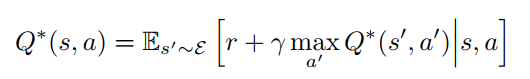
\includegraphics[width=1\linewidth]{bellman}}
    \caption{Bellman Equation - функция поведения игрока}
\end{figure}

Помимо этого, с определённой вероятностью, которая уменьшается после каждой игры, вместо наиболее выгодного действия выбирается случайное из возможных. После каждой игры выбираются случайные наборы действий для корректировки весов нейронной сети, то есть основная задача нейронной сети предсказать какое действие приведёт к максимальному значению Q функции в следующий момент времени. Данный метод называется Q-Learning. После реализации алгоритма авторы статьи сравнили полученные результаты с результатами других способов обучения искусственного интеллекта. Q-Learning в большинстве игр оказался лучшим.
\subsection{Обзор существующих технологий для реализации проекта}
В связи с развитием машинного обучения в последние годы появилось множество вспомогательных библиотек, которые инкапсулируют реализацию моделей нейронной сети, позволяя очень быстро протестировать идею без постоянного написания основного каркаса нейронной сети.

Одной из самых популярных библиотек машинного обучения является TensorFlow[9], разрабатываемая компанией Google. TensorFlow – это программная библиотека с открытым исходным кодом для численных вычислений с использованием графов потоков данных (data flow graphs). Узлы в таком графе представляют математические операции, в то время, как грани представляют передачу данных (многомерных массивов) между узлами. Гибкая архитектура, на основе которой построен TensorFlow, позволяет разворачивать вычисления на одном или нескольких CPU или GPU (т.е. на центральном или графическом процессоре) на обычном персональном компьютере, сервере или даже мобильном устройстве используя единый программный интерфейс (API).  В одной из статей рассматриваются основные возможности данного программного решения[2]. Автор реализует логистическую регрессию и сравнивает время выполнения с результатом библиотеки scikit-learn. TensorFlow оказывается гораздо быстрее – 17c против 3 мин., и точнее в предсказании на тестовой выборке – 92% против 91.8%. На данном примере отмечается, что принципиальным отличием TensorFlow (далее – TF) от scikit-learn в том, что определение порядка вычислений и собственно само вычисление разнесено на отдельные шаги, т.е., определяя последовательность действий в TF, на самом деле формируется граф операций, а само вычисление графа будет происходить позже, на уже конкретных физических устройствах (CPU, GPU или отдельных компьютерах), что приводит к ускорению вычислений. 

Далее автор реализует feed-forward нейронную сеть, отмечая, что основная сложность нейронных сетей заключена в обратном распространении ошибки, однако, работая с TF об этом не приходится задумываться, потому что в нем реализован обобщенный алгоритм обратного распространения ошибки, т.е. такой алгоритм, который применим к любым доступным операциям (будь то умножение матриц или операция свертки для свёрточных нейронных сетей). Для обучения используется 55000 изображений, для валидации 5000, в качестве тестовой выборки 10000 изображений. В результате выполнения отмечается, что TensorFlow выполняется в 6 раз быстрее библиотеки Theano. Помимо этого, TensorFlow предоставляет встроенные средства визуализации, которые повышают наглядность обучаемых моделей.

Несмотря на то, что TensorFlow подходит как для широкого набора техник машинного обучения, так и для глубинного обучения, библиотека может быть довольно сложна в понимании особенно для тех разработчиков, которые только начинают знакомство с данными областями исследования. Альтернативой является «надстройка» Keras [10], которая предоставляет удобный и простой в использовании программный интерфейс для обучения глубоких нейронных сетей. Keras не является самостоятельной системой, а работает поверх Theano, TensorFlow или CNTK. В 2016 году Keras включили в состав TensorFlow[10]. Помимо этого, все классы являются максимально расширяемыми и модульными, благодаря этому библиотека представляет широкий функционал возможностей по решению сложных практических задач.
\subsection*{Выводы}
\addcontentsline{toc}{subsection}{Выводы}
В результате обзора литературы были изучены различные реализации нейронных сетей для построения логики игрового противника. Игра в монополию является марковским случайным процессом [7], следовательно, для обучения искусственного интеллекта был выбран алгоритм Q-Learning.

Были рассмотрены основные средства реализации нейронных сетей в языке Python, в результате чего была выбрана реализация с применением библиотеки Keras.
\end{Large}
\setlength{\parskip}{0cm}
\begin{Large}
\newpage
\section{Требования к системе}
\subsection{Основные правила игры <<Монополия>>}
Для правильного определения требований к разрабатываемой системе необходимо сначала выделить основные правила разрабатываемой игры.

«Монополия» - это экономическая пошаговая стратегия. Главная цель игры – рационально использовать полученный вначале капитал, который выдаётся всем игрокам в равном объёме, и привести к банкротству других участников. Пошаговый игровой процесс разбивается на ходы, каждый игрок ходит по очереди. Игрок перемещается по игровому полю в зависимости от количества очков, выпавшему на кубиках. Если выпал дубль, то игрок повторяет свой ход. В зависимости от клетки, на которую игрок попадает совершаются разнообразные действия.

Помимо перемещения и выполнения действий, приписанных этой клетке игрок вправе:
\begin{spacing}{0.9}
\begin{enumerate}
    \item Участвовать в аукционах недвижимости, которую отказывались покупать другие игроки 
    \item Улучшать свои владения посредством покупки домов для увеличения арендной платы, которая платится другими игроками при попадании на клетку недвижимости
    \item Продавать дома по необходимости
    \item Закладывать участки недвижимости при отсутствии денег
    \item Выкупать свои участки из залога
\end{enumerate}
\end{spacing}

\textbf{Объекты игры}

На игровом поле расположены клетки. В начале игры каждый игрок располагается на начальной клетке «Вперёд». Всего клетки могут быть разных типов:
\begin{spacing}{0.9}
\begin{enumerate}
    \item Улица – поле доступное для покупки, улицы делятся на группы по цвету, завладев одним цветом, игрок вправе купить дом на данной улице. Если игрок попадает на данное поле, и оно не принадлежит никому, то он вправе его купить за указанную стоимость. Если игрок попадает на данном поле, и оно принадлежит другому игроку, то игрок платит арендную плату этому игроку в зависимости от уровня развития данной улицы. Аналогичная логика используется на полях «Коммунальное предприятие» и «Железнодорожная станция». 
    \item Коммунальное предприятие – поле доступное для покупки, арендная плата на нем считается в зависимости от количества выпавших очков
    \item Железнодорожная станция – поле доступное для покупки, арендная плата на нём считается в зависимости от количества купленных полей данного типа у владельца поля.
    \item «Шанс» и «Общественная казна» -  поля, на которых игрок должен выполнить действие, которое случайно выберет игра.
    \item Бесплатная стоянка – поле, на котором ничего не происходит
    \item «Налог» - игрок обязан выплатить определенную сумму налога
\end{enumerate}
\end{spacing}

\textbf{Тюрьма}

Игрок отправляется в Тюрьму, если:
\begin{spacing}{0.9}
\begin{enumerate}
    \item Остановится на поле «Отправляйтесь в Тюрьму» 
    \item Игрок взял карточку «Шанс» или «Общественная казна», на которой написано «Отправляйтесь в Тюрьму»
    \item У игрока выпало одинаковое число очков на обоих кубиках три раза подряд за один ход
\end{enumerate}
\end{spacing}

Ход игрока оканчивается, когда его отправляют в Тюрьму. 

Чтобы выйти из Тюрьмы, игроку необходимо:
\begin{spacing}{0.9}
\begin{enumerate}
    \item Заплатить штраф в размере 50 рублей и продолжить игру
    \item Попытаться выбросить дубль
\end{enumerate}
\end{spacing}

После того, как игрок пропустит три хода, находясь в Тюрьме, он должен выйти из неё и уплатить 50 тыс. рублей, прежде чем сможет переместиться на такое число полей, которое выпало на кубиках. 

Находясь в Тюрьме, игрок может получать арендную плату за недвижимость, если она не заложена. Если игрок не был «отправлен в Тюрьму», а просто остановился на поле «Тюрьма» в ходе игры, то он не платит никакого штрафа.

\textbf{Залог}

Если у игрока не хватает денег, то он вправе заложить определенное поле. Для этого, сначала продаются все дома, расположенные на данной клетке, если такие имеются и затем игроку передаётся половина от стоимости клетки. 

После этого, если другой игрок окажется на данной клетке, то арендная плата взыматься не будет. Однако с других клеток плата взыматься будет.

Для того, чтобы выкупить данную клетку, игроку необходимо внести половину стоимости клетки + 10\%.

\textbf{Покупка домов}

Если игрок купил всю цветовую группу клеток, то он монополизировал данную цветовую группу и вправе строить дома на ней. Однако, если хоть одна клетка из цветовой группы заложена, то игрок теряет данную возможность.

Постройка домов увеличивает арендную плату. На одной клетке можно построить максимум 4 дома

\textbf{Банкротство}

Если игрок должен Банку или другому игроку больше денег, чем может получить по своим активам, то он объявляется банкротом, и выбывает из игры

Если игрок должен Банку, Банк получает все деньги игрока. Затем вся недвижимость обанкротившегося игрока продаётся с аукциона.

Если игрок должен другому игроку, все дома банкрота продаются, полученные средства передаются игроку, обанкротившему его, как и вся недвижимость, включая заложенную.
\subsection{Функциональные требования}
\begin{spacing}{0.9}
\begin{enumerate}
    \item Система игра «Монополия» должна реализовывать основные правила настольной игры 
    \item Система игра «Монополия» должна поддерживать локальный многопользовательский режим
    \item Система игра «Монополия» должна правильно определять победителя партии.
\end{enumerate}
\end{spacing}
\subsection{Нефункциональные требования}
\begin{spacing}{0.9}
\begin{enumerate}
    \item Система игра «Монополия» должна быть написана на языке Python 
    \item Система игра «Монополия» должна поддерживать как реальных игроков, так и ботов
    \item Система игра «Монополия» должна реализовывать текстовый интерфейс
\end{enumerate}
\end{spacing}
\subsection{Диаграмма вариантов использования}
Система представляет собой программу, реализующую игру «Монополия».

Единственным актёром системы является игрок.
\begin{figure}[h!]
    \center{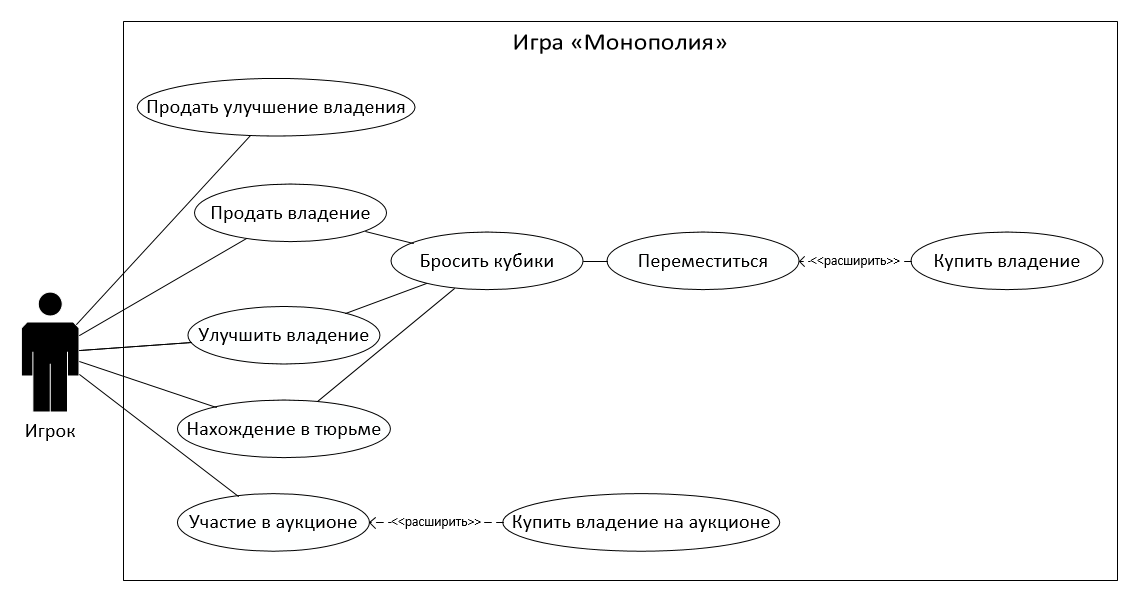
\includegraphics[width=1\linewidth]{use-case.png}}
    \caption{Диаграмма вариантов использования}
\end{figure}

Определим основные варианты использования системы игра «Монополия». Пользователю доступны следующие функции:
\begin{enumerate}
    \item \textit{Продать улучшение владения} – игрок может продать ненужные улучшения его владений во время своего хода для получения дополнительного заработка
    \item \textit{Продать владение} – игрок может продать ранее приобретённые владения
    \item \textit{Улучшить владение} – игрок может улучшить приобретённое владение, если цветовая группа владения находится под контролём его монополии
    \item \textit{Нахождение в тюрьме} – игрок может находиться в тюрьме определённое количество ходов
    \item \textit{Участие в аукционе} – игрок может участвовать в уникальном событии – аукционе
    \item \textit{Бросить кубики} – игрок бросает кубики для определения количества клеток для перемещения
    \item \textit{Переместиться} – игрок перемещается на выпавшее количество очков
    \item \textit{Купить владение} – игрок может купить владение, на которое он попал, если оно не принадлежит никому
\end{enumerate}
\subsection{Спецификация основных вариантов использования}
\newpage
\begin{table}[h!]
\caption{Спецификация прецедента <<Нахождение в тюрьме>>}
\begin{tabular}{|l|}
    \hline
    \textbf{UseCase: Нахождение в тюрьме}\\
    \hline
    \textit{Аннотация:}\ Нахождение игрока в тюрьме\\
    \hline
    Главные актеры: Игрок \\
    \hline
    Второстепенные актеры: Нет \\
    \hline
    Предусловия: Игрок находится в тюрьме \\
    \hline
    Основной поток: \\
        1)Система проверяет количество ходов, проведенных в тюрьме игроком \\
        2)Игроку предлагается купить выход из тюрьмы \\
        3)Игрок выплачивает штраф за выход из тюрьмы \\
        4)Игрок выходит из тюрьмы \\
    \hline
    Постусловия: Игрок вышел из тюрьмы\\
    \hline
    Альтернативные потоки:\\
    2А Игрок отказался покупать выход из тюрьмы\\
    1)Игрок остаётся в тюрьме\\
    1А Игрок слишком долго находится в тюрьме\\
    1)Игрок выплачивает штраф за выход из тюрьмы\\
    2)Игрок выходит из тюрьмы\\
    4А Игрок не в состоянии оплатить штраф за выход из тюрьмы\\
    1)Система предлагает игроку продать владения\\
    2)Игрок продаёт владения\\
    3)Игрок выплачивает штраф за выход из тюрьмы\\
    4)Игрок выходит из тюрьмы\\
    4А 1А Игрок не имеет владений, игрок отказался продавать владения\\
    1)Игрок становится банкротом\\
    2)Все владения игрока продаются на аукционе\\
    \hline
\end{tabular}  
\end{table}
\newpage
\begin{table}[h!]
    \caption{Спецификация прецедента <<Купить владение>>}
    \begin{tabular}{|l|}
        \hline
        \textbf{UseCase: Купить владение}\\
        \hline
        \textit{Аннотация:}\ Нахождение игрока в тюрьме\\
        \hline
        Главные актеры: Игрок \\
        \hline
        Второстепенные актеры: Нет \\
        \hline
        Предусловия: Владение никому не принадлежит и доступно для покупки \\
        \hline
        Основной поток: \\
            1)Система предлагает купить владение \\
            2)Игрок решает купить владение \\
            3)Система проверяет возможность покупки владения игроком \\
            4)Игрок завладевает ячейкой\\
        \hline
        Постусловия: Ход передаётся следующему игроку\\
        \hline
        Альтернативные потоки:\\
        2А Игрок отказывается от покупки, 3А Игроку не хватает денег для покупки\\
        1)Ячейка выставляется на аукционе\\
        2)Все игроки оповещаются о начале аукциона\\
        \hline
    \end{tabular}  
\end{table}
\subsection*{Выводы}
\addcontentsline{toc}{subsection}{Выводы}
В процессе анализа требований был определен основной актер системы, варианты использования системы, сформулированы основные функциональные и нефункциональные требования, предъявляемые к разрабатываемой системе.
\end{Large}
\newpage
\setlength{\parskip}{0cm}
\begin{Large}
\section{Архитектура системы}
Опишем архитектуры системы, основанную на требованиях, сформулированных в предыдущей главе
\subsection{Диаграмма классов}
\begin{figure}[h]
    \center{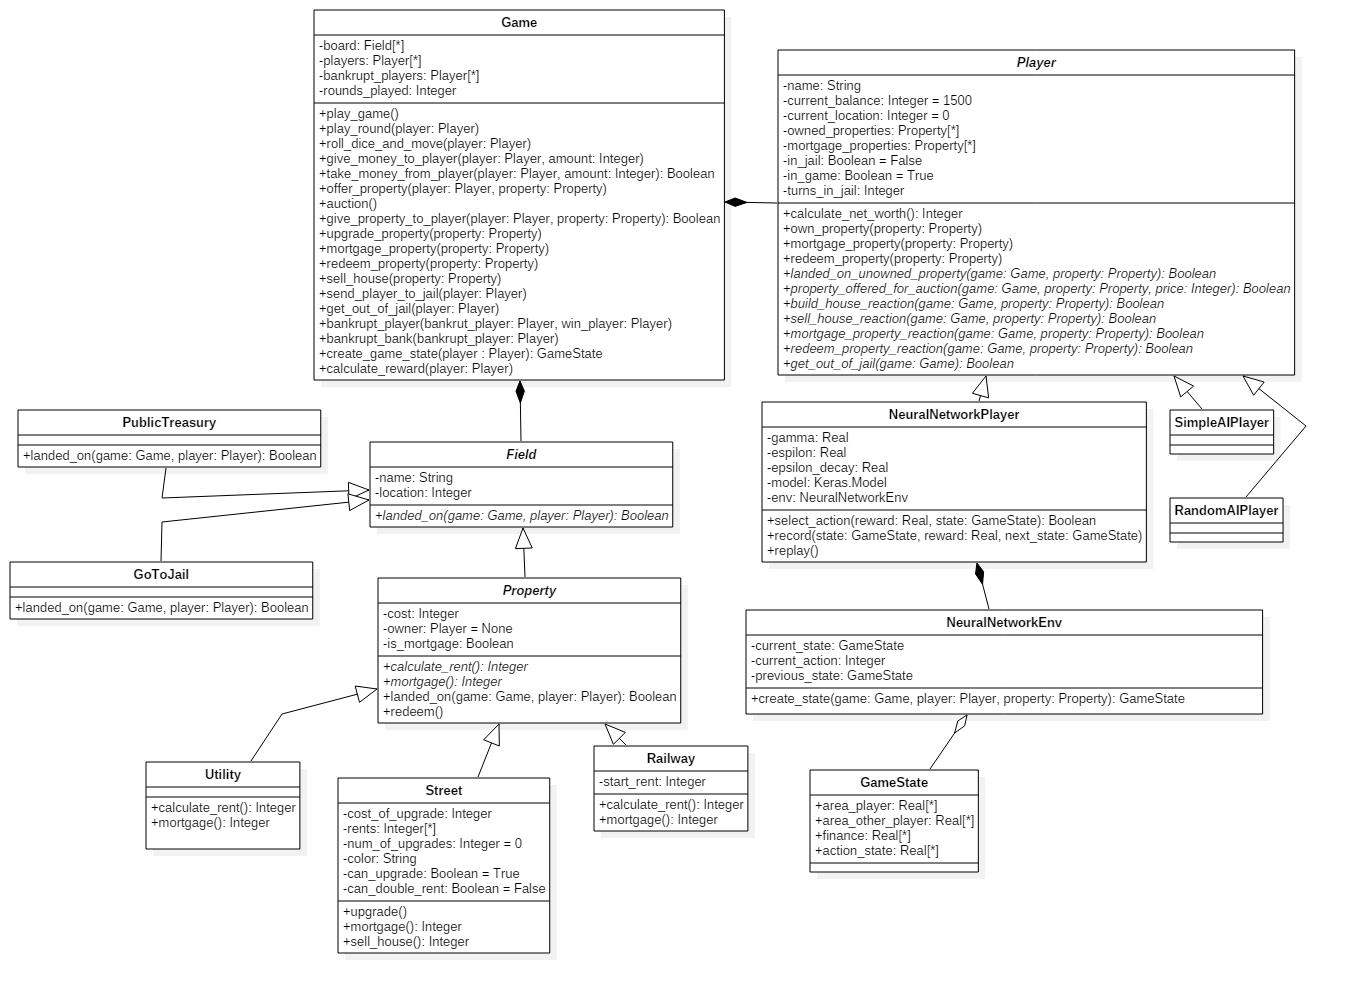
\includegraphics[width=1\linewidth]{class.png}}
    \caption{Диаграмма классов}
\end{figure}
Далее будет описана семантика основных классов программной части и перечислены их функции.
\begin{spacing}{0.9}
\begin{enumerate}
    \item Game - основной класс, в котором реализована логика игры
    \item Field – абстрактный класс поля
    \item Property – абстрактный класс поля, которым может владеть игрок
    \item Chance, Forward, FreeParking, GoToJail, Jail, Tax – поля, которыми нельзя владеть, но которые реализуют различные игровые механики
    \item Utility – класс, реализующий поля «Коммунальное предприятие»
    \item Railway – класс, реализующий поля «Железная дорога»
    \item Street – класс, реализующий поля улиц
    \item Player – абстрактный класс, реализующий интерфейс для разработки ботов, путём реализации логики ответа на события, происходящие в игре
    \item NeuralNetworkPlayer – класс, реализующий нейронную сеть
    \item NeuralNetworkEnv – класс, сохраняющий и формирующий состояния для нейронной сети
    \item RandomAIPlayer – класс, реализующий случайное реагирование на события в игре
    \item SimpleAIPlayer – класс, реализующий простейшую логику бота
    \item GameState – класс, реализующий структуру игрового состояния
\end{enumerate}
\end{spacing}
\subsection{Блок-схема алгоритма аукциона}
Механика аукциона является одной из важнейших в «Монополии», однако полноценная реализация данной механики и удобное использование её средствами нейронной сети является затруднительной и ресурсоёмкой задачей. Для удобного взаимодействия ботов с механикой аукциона был разработан алгоритм, блок-схема которого представлена на рис 4.
\begin{figure}[h!]
    \center{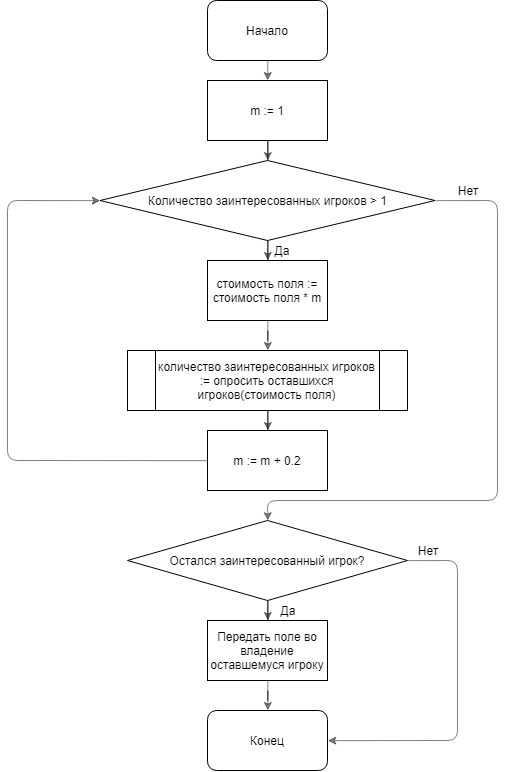
\includegraphics[scale=0.85]{auction.png}}
    \caption{Блок-схема аукциона}
\end{figure}
\newpage
\subsection{Определение характеристик состояния игры и действий игрока}
Для успешного проектирования нейронной сети нужно сформулировать данные, которые будут формировать текущее состояние игры.

Первые 10 значений характеризуют процент владения недвижимостью игровым агентом, представляющим нейронную сеть (8 различных цветов улиц, коммунальные предприятия и железные дороги)

Для улиц значения можно описать таким образом:
\begin{spacing}{0.9}
\begin{enumerate}
    \item 0 – игрок не владеет данным цветом
    \item 0 < xi < 0.6 – игрок владеет хотя бы одним полем данного цвета
    \item 0.6 – игрок монополизировал данное поле
    \item 0.6 < xi < 1 – игрок построил хотя бы один дом на поле данного
    \item 1 – игрок полностью застроил владения данного цвета 
\end{enumerate}
\end{spacing}
Для коммунального предприятия значение описываются так:
\begin{spacing}{0.9}
\begin{enumerate}
    \item 0 – игрок не владеет ни одним полем данного типа
    \item 0.5 – игрок владеет одним полем данного типа
    \item 1 – игрок монополизировал поля данного типа
\end{enumerate}
\end{spacing}
Для железной дороги значения описываются так:
\begin{spacing}{0.9}
\begin{enumerate}
    \item 0 – игрок не владеет ни одним полем данного типа
    \item 0.25 – игрок владеет одним полем
    \item 0.5 – игрок владеет двумя полями 
    \item 0.75 – игрок владеет тремя полями
    \item 1 – игрок монополизировал данный тип поля
\end{enumerate}
\end{spacing}
Следующие 10 значений характеризуют процент владения недвижимостью другими игроками, который рассчитывается по принципу, описанному выше

Следующие 4 значения характеризуют финансовую составляющую агента:
\begin{enumerate}
    \item Отношение активов, принадлежащих агенту к общим активам рассчитываются по формуле 
    \begin{equation}
        x_i = \frac{b_1+n_1}{\sum_{i=1}^{num\_players}b_i + \sum_{i=1}^{num\_players}n_i}
    \end{equation}
    где b – баланс игрока, n – текущая ценность купленной недвижимости
    \item Отношение текущего баланса к начальному, которое рассчитывается по формуле
    \begin{equation}
        x_i = \frac{\frac{b}{1500}}{1+\frac{b}{1500}}
    \end{equation}
    где b -  текущий баланс игрока
    \item Отношение максимальной возможной растраты на аренду/налог к текущему балансу, которое рассчитывается по формуле
    \begin{equation}
        x_i = \frac{\frac{maxrent-b}{b}}{1+|\frac{maxrent-b}{b}|}
    \end{equation}    
    где maxrent – максимально возможная растрата, b – текущий баланс
    \item Отношение купленной недвижимости к общей купленной недвижимости, которое рассчитывается по формуле
    \begin{equation}
        x_i = \frac{p_1}{\sum_{i=1}^{num\_players}p_i}
    \end{equation}
\end{enumerate}

Последнее значение характеризует позицию недвижимости по которому требуется решение, которое формируется в значениях [0, 1]. Например, для поля синего цвета значение будет 0.2.

Для определения размера выходного слоя нейронной сети необходимо определить возможные действия в игре, они будут формировать вектор Action. Предполагается 3 действия:
\begin{spacing}{0.9}
\begin{enumerate}
    \item Купить – купить владение, купить дом во владении, выкупить дом из залога, купить владение на аукционе
    \item Продать – продать дом, заложить владение
    \item Ничего не делать
\end{enumerate}
\end{spacing}
\subsection{Архитектура проектируемой нейронной сети}
Была выбрана следующая архитектура нейронной сети (рис. 4), позволяющая оптимально сочетать в себе скорость обучения и точность решения предоставленных задач.

Нейронная сеть имеет 4 слоя и выглядит следующим образом:
\begin{spacing}{0.9}
\begin{enumerate}
    \item Входной слой определяется размерностью вектора State, описанному в главе ранее.
    \item Первый скрытый слой содержит 200 нейронов. У данного слоя используется функция активации ReLU.
    \item Второй скрытый слой содержит 75 нейронов. У данного слоя используется функция активации ReLU.
    \item Выходной слой определяется размерностью вектора Action. В каждом нейроне на выходе будет значение предполагаемой награды при совершении подобного действия.
\end{enumerate}
\end{spacing}
\newpage
\begin{figure}[h]
    \center{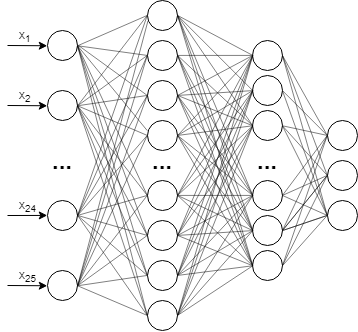
\includegraphics[scale=0.75]{nn.png}}
    \caption{Архитектура нейронной сети}
\end{figure}
\subsection{Функция награды}
Основной задачей игры является завладеть большим количеством полей чем противники и при этом иметь достаточно количество денег для непредвиденных растрат. Для успешного обучения нейронной сети методом Q-learning необходимо сформулировать функцию награды, которая будет выдаваться нейронной сети после каждого выполненного хода. 
\begin{figure}[h!]
    \center{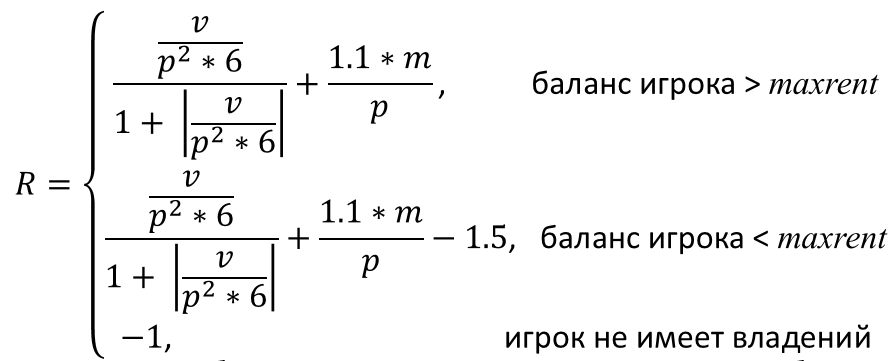
\includegraphics[scale=0.65]{reward.png}}
    \caption{Функция награды}
\end{figure}

где v – разница между приобретенными владениями игрока и приобретенными владениями других игроков, p – количество игроков, m – отношение баланса игрока к балансу всех игроков. Награда игрока будет находиться в значениях [-1;1].
\subsection*{Выводы}
\addcontentsline{toc}{subsection}{Выводы}
В соответствии с требованиями была спроектирована структура разрабатываемой системы, были определены характеристики состояния системы и выделены возможные действия игрока. 

В соответствии с характеристиками состояния и возможных действий игрока была спроектирована нейронная сеть и определена функция награды 
\end{Large}
\newpage
\section{Реализация системы}
\subsection{Обзор инструментов для разработки}
Для создания игры «Монополия» был выбран язык Python, который на данный момент является передовым решением для машинного обучения, помимо этого он достаточно прост в освоении и позволяет быстро реализовать необходимые алгоритмы. Для реализации нейронной сети была выбрана библиотека Keras, которая представляет собой простой и удобный интерфейс для обучения нейронных сетей. В качестве среды разработки была выбрана PyCharm 2018.1
\subsection{Реализация интерфейса для создания ботов}
Игра «Монополия» включает в себя интерфейс для создания ботов. Для того, чтобы разработанный бот являлся полноценным актёром системы он должен реализовывать следующие методы:
\begin{enumerate}
    \item \textit{landed\_on\_unowned\_property (self, game, field)} – метод, вызываемый, когда игрок попадает на поле, не принадлежащее никому. Возвращает true – если покупка одобрена, false – покупка не одобрена
    \item \textit{property\_offered\_for\_auction (self, game, field, price)} - метод, вызываемый, когда игрок участвует в аукционе. Возвращает true – если цена устраивает, false – если цена не устраивает, и игрок хочет выйти из аукциона
    \item \textit{build\_house (self, game, field)} – метод, вызываемый, когда игроку предлагается купить дом на поле. Возвращает true – если покупка одобрена, false – покупка не одобрена
    \item \textit{sell\_house (self, game, field)} – метод, вызываемый, когда игроку предлагается продать дом на поле. Возвращает true – если продажа одобрена, false – продажа не одобрена
    \item \textit{mortgage\_property (self, game, field)} – метод, вызываемый, когда игроку предлагается заложить своё поле. Возвращает true – если залог одобрен, false – залог не одобрен
    \item \textit{redeem\_property (self, game, field)} – метод, вызываемый, когда игроку предлагается выкупить своё поле из залога. Возвращает true – если выкуп одобрен, false – выкуп не одобрен
    \item \textit{get\_out\_of\_jail (self, game)} – метод, вызываемый, когда игрок находится в тюрьме и ему предлагается выйти из тюрьмы, оплатив выкуп. Возвращает true – если выкуп одобен, false – выкуп не одобрен.
\end{enumerate}
\subsection{Реализация Q-обучения нейронной сети}
Для реализации обучения нейронной сети были сделаны несколько методов:
\begin{enumerate}
    \item \textit{select\_action (self, state)} – выбор следующего действия нейронной сети, исходя из игрового состояния
    \item \textit{record (self, state,action, reward, next\_state, done)} – запись текущих действий нейронной сети
    \item \textit{replay(self)} – функция обучения нейронной сети
\end{enumerate}
\begin{figure}[h!]
    \center{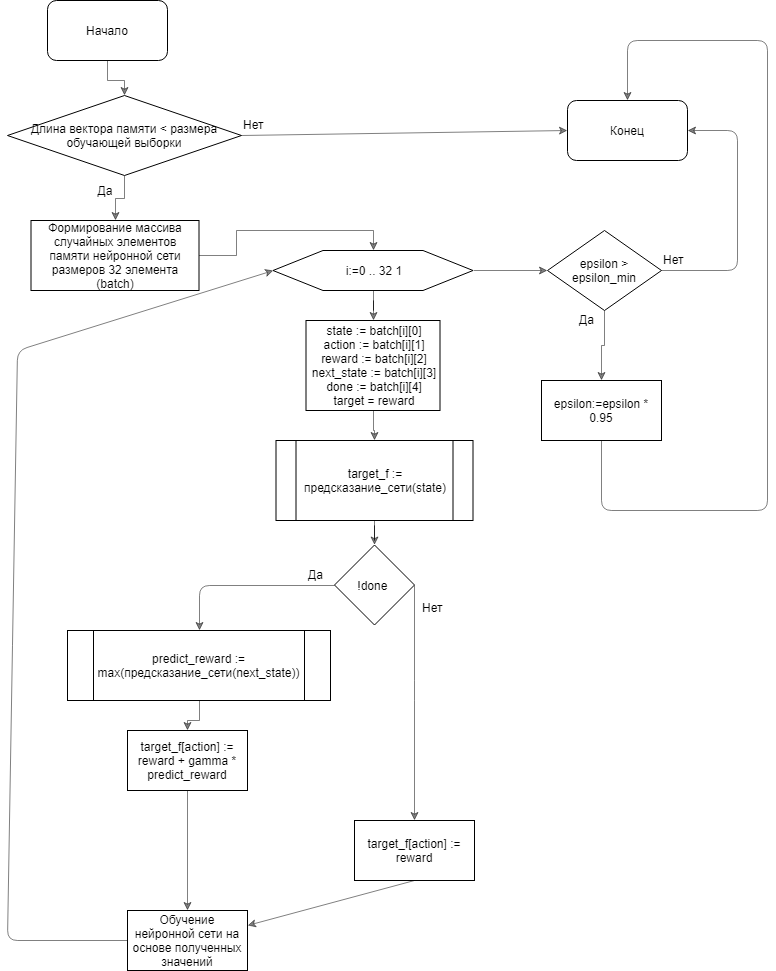
\includegraphics[scale=0.85]{bnn.png}}
    \caption{Блок-схема обучения нейронной сети}
\end{figure}
\newpage
\subsection{Реализация игровых ботов}
Для удобного обучения и тестирования нейронной сети была реализована простая логика противников. 

Первый тип противника работает по принципу случайного поведения игрока, то есть на любое предлагаемое действие он реагирует случайным образом.

Второй тип противника реализует простое поведение игрока. Основные правила, которых он придерживается:
\begin{enumerate}
    \item Согласиться с покупкой, если баланс игрока – стоимость покупки> 350
    \item Согласиться с продажей, если баланс игрока меньше 150
    \item Ничего не делать, если баланс находится в промежутке между 150 и 350.
\end{enumerate}
\subsection*{Выводы}
\addcontentsline{toc}{subsection}{Выводы}
На основе разработанной архитектуры было реализована система игра «Монополия». Выполнена реализация интерфейса для создания ботов и обучения нейронной сети.
\newpage
\section{Тестирование}
\subsection{Функциональное тестирование}
\begin{table}[!h]
    \caption{Функциональное тестирование}
    \begin{tabularx}{450pt}{|l|X|X|X|X|}
        \hline
        \textnumero & Название теста & Действия тестировщика & Ожидаемый результат & Прохождение теста\\
        \hline
        1 & Покупка недвижимости & Соглашается с предложением о покупке недвижимости & Недвижимость переходит во владение игрока. Со счёта игрока снимается стоимость недвижимость & Да\\
        \hline
        2 & Отказ от покупки недвижимости & Отказывается от предложения о покупке недвижимости & Недвижимость выставляется на аукцион & Да\\
        \hline
        3 & Залог недвижимости & Соглашается с предложением о залоге недвижимости & Недвижимость становится заложенной. Игроку перечисляются средства на счёт & Да\\
        \hline
        4 & Выкуп недвижимости & Соглашается с предложение о выкупе недвижимости & Недвижимость снова становится активной. Со счёта игрока снимается стоимость выкупа & Да\\
        \hline
    \end{tabularx}  
\end{table}
\subsection{Тестирование обучения нейронной сети}
Перед стартом обучения нейронной сети было протестировано преимущество противника, реализующего простейшую логику, перед противником, реализующим случайное поведение. Отношение побед оказалось 97 на 3 в пользу простой логики.

Нейронная сеть обучалась при параметрах:
\begin{spacing}{0.9}
\begin{enumerate}
    \item learning\_rate = 0.01
    \item gamma = 0.95
    \item размер памяти нейронной сети = 100
    \item размер обучающей выборки = 32
    \item epsilon = 1, epsilon\_min = 0.1, epsilon\_decay = 0.995
\end{enumerate}
\end{spacing}

\subsubsection*{Обучение нейронной сети в игре против случайного поведения противника}
\newpage
\begin{figure}[h!]
    \center{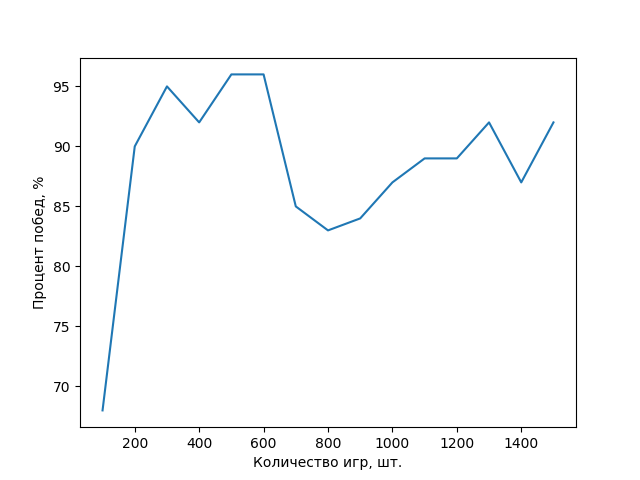
\includegraphics[scale=0.75]{rnn1.png}}
    \caption{Изменение процента побед в игре против случайного поведения противника}
\end{figure}
\begin{figure}[h!]
    \center{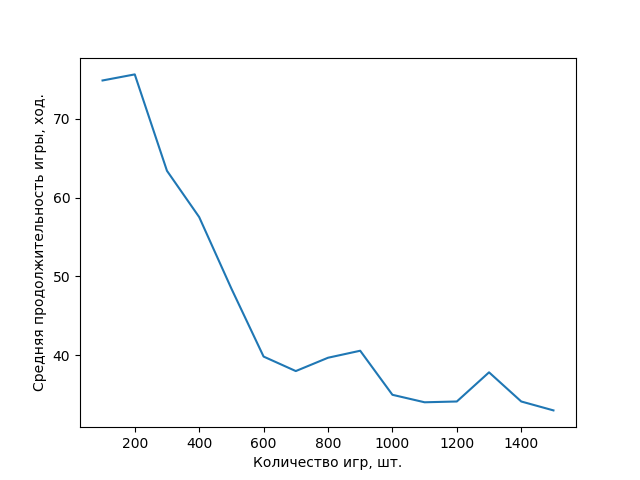
\includegraphics[scale=0.75]{rnn2.png}}
    \caption{Изменение средней продолжительности игры в игре против случайного поведения противника}
\end{figure}
\subsubsection*{Обучение нейронной сети против простого поведения противника}
\begin{figure}[h!]
    \center{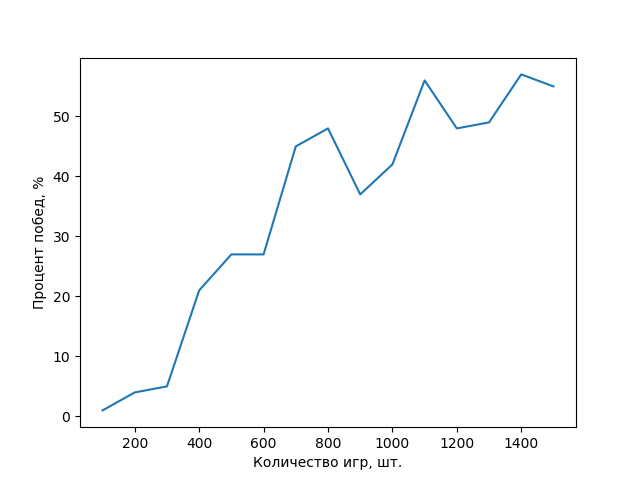
\includegraphics[scale=0.75]{snn1.png}}
    \caption{Изменение процента побед в игре против простого поведения противника}
\end{figure}
\begin{figure}[h!]
    \center{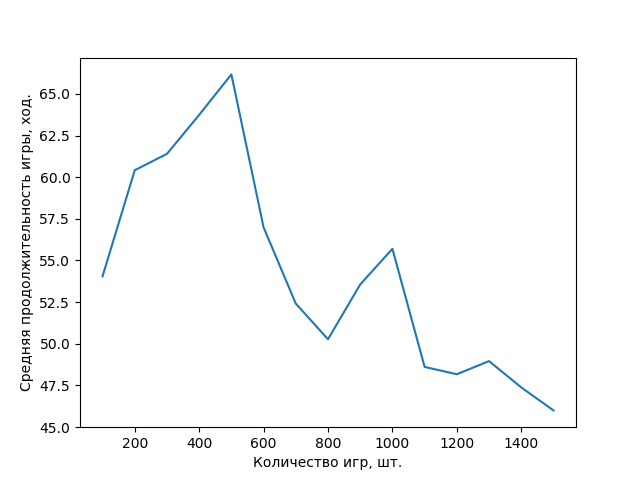
\includegraphics[scale=0.75]{snn2.png}}
    \caption{Изменение средней продолжительности игры в игре против простого поведения противника}
\end{figure}
\subsection*{Выводы}
\addcontentsline{toc}{subsection}{Выводы}
В ходе тестирования были проведены несколько экспериментов, которые обнаружили достоинства и недостатки алгоритма Q-обучения. 

Достоинства:
\begin{spacing}{0.9}
\begin{enumerate}
    \item Отсутствие необходимости формирования обучающей выборки перед началом обучения
    \item Возможность формирования стратегии игрока в функции награды
\end{enumerate}
\end{spacing}

Недостатки:
\begin{spacing}{0.9}
\begin{enumerate}
    \item Возможное переобучение
    \item Сложность формирования действий нейронной сети, подлежащих обучению
    \item Сложность определения функции награды
\end{enumerate}
\end{spacing}

Для улучшения процента побед предлагается:
\begin{spacing}{0.9}
\begin{enumerate}
    \item Изменение функции награды
    \item Улучшение алгоритма выбора совершенных действий нейронной сети, подлежащих обучению.
\end{enumerate}
\end{spacing}
\newpage
\section*{Заключение}
\addcontentsline{toc}{section}{Заключение}
В ходе проделанной работы были решены следующие задачи:
\begin{spacing}{0.9}
\begin{enumerate}
    \item Изучены основные методы обучения нейронной сети для игр 
    \item Определены требования к системе игра «Монополия»
    \item Разработана структура игры и архитектура нейронной сети
    \item Реализована игра «Монополия»
    \item Реализована нейронная сеть 
    \item Протестированы функционал игры и реализация нейронной сети
\end{enumerate}
\end{spacing}
\newpage
\addcontentsline{toc}{section}{Литература}
\begin{thebibliography}{99}
\bibitem{1} Коваленко А.С., Ковалевский В.Н. Построение логики игрового противника путём использования машинного обучения // Новые задачи технических наук и пути их решения. Сборник статей Международной научно-практической конференции, 2017.  С. 140-144.
\bibitem{2} Латкин И.И. Обзор возможностей TensorFlow для решения задач машинного обучения // Молодежный научно-технический вестник, 2016. 
\bibitem{3} Созыкин А. В. Обзор методов обучения глубоких нейронных сетей // Вестник Южно-Уральского государственного университета. Серия: Вычислительная математика и информатика, 2017. С. 28-49
\bibitem{4} Сотников И.Ю., Григорьева И.В. Адаптивное поведение программных агентов в мультиагентной компьютерной игре // Вестник Кемеровского государственного универститета, 2014. С. 65-71
\bibitem{5} Шампандар А. Искусственный интеллект в компьютерных играх. М.: Вильямс, 2007 - 768 с
\bibitem{6} Mnih, Volodymyr, Kavukcuoglu, Koray, Silver, David, Graves, Alex, Antonoglou, Ioannis, Wierstra, Daan, and Riedmiller, Martin. Playing atari with deep reinforcement learning // NIPS Deep Learning Workshop. 2013. pp. 1-9
\bibitem{7} Robert B Ash, Richard L Bishop, ‘Monopoly as a markov process’, Mathematics Magazine, 45(1), 1972, pp. 26–29
\bibitem{8} Tariq Rashid. Make your own neural network, 2015. 240 p
\bibitem{9} Официальный сайт TensorFlow. [Электронный ресурс] URL: https://www.tensorflow.org (дата обращения 21.03.2018).
\bibitem{10} Keras: The Python Deep Learning library [Электронный ресурс] URL: http://keras.io (дата обращения 21.03.2018)
\end{thebibliography}
\end{document}